% !TEX root = ../main.tex
% 本文件由 build-tex.sh 从 06-DSP指南-第6章中译.md 生成，改内容请改 md 后重新生成

\chapter{卷积}\label{ch-06}

卷积(convolution)是把两个信号组合成第三个信号的一种数学方法。它是数字信号处理中最重要的一项技术。利用冲激分解的策略，系统用一个叫冲激响应(impulse
response)的信号来描述。卷积之所以重要，是因为它把我们关心的三个信号联系在一起：输入信号、输出信号和冲激响应。本章从两个不同的角度介绍卷积，分别叫输入端算法(input
side algorithm)和输出端算法(output side algorithm)。卷积为 DSP
提供了数学框架，本书没有比它更重要的内容了。

\section{冲激函数与冲激响应}

上一章讲了怎样把一个信号分解成一组叫冲激(impulse)的分量。冲激是除一个非零点外全为零的信号。实际上，冲激分解提供了一种一次分析信号一个采样的方法。上一章还介绍了
DSP
的基本概念：把输入信号分解成简单的相加分量，让每个分量通过线性系统，再把得到的输出分量合成（相加）。这种分而治之的做法得到的信号，和把原始信号直接通过系统得到的信号完全相同。可能的分解虽然很多，但构成信号处理骨架的只有两种：冲激分解和傅里叶分解。使用冲激分解时，这个过程可以用一种叫卷积的数学运算来描述。本章（以及后面大多数章节）只讨论离散信号。卷积也适用于连续信号，但数学更复杂。第
13 章会讲连续信号怎样处理。

图 6-1 定义了 DSP 中两个重要的术语。第一个是冲激函数(delta
function)，用希腊字母 delta 表示，记作
δ{[}n{]}。冲激函数是归一化的冲激，即第 0 个采样的值为
1，其余所有采样的值都为 0。因此，冲激函数也常被称为单位冲激(unit
impulse)。

图 6-1
定义的第二个术语是冲激响应。顾名思义，冲激响应就是输入为冲激函数（单位冲激）时系统输出的信号。两个系统只要有任何不同，它们的冲激响应就不同。正如输入和输出信号常被叫做
x{[}n{]} 和 y{[}n{]}，冲激响应通常用符号 h{[}n{]}
表示。当然，如果有更具描述性的名字也可以换，比如可以用 f{[}n{]}
来表示一个滤波器(filter)的冲激响应。

\begin{figure}[htbp]
\centering
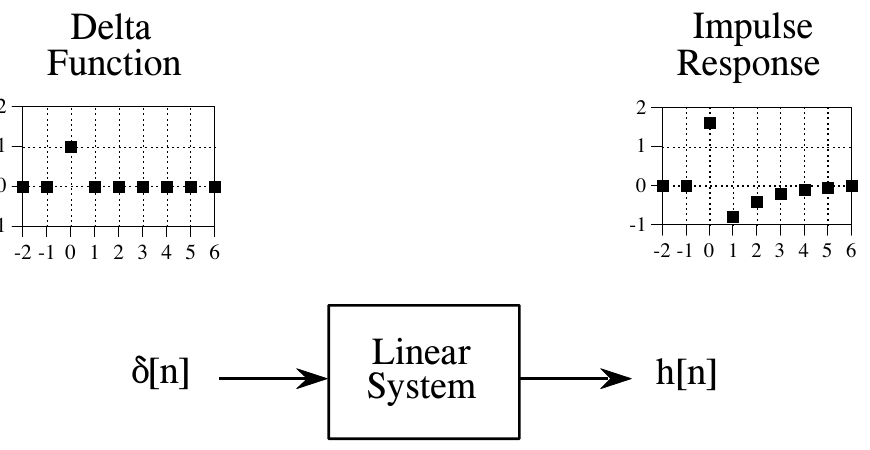
\includegraphics[width=0.725\linewidth,height=0.8\textheight,keepaspectratio]{assets/ch06/fig6-01.png}
\caption*{\textbf{图 6-1　冲激函数和冲激响应的定义。} 冲激函数是归一化的冲激：除第
0 个采样的值为 1 外，所有采样的值都为 0。用希腊字母 delta，即
δ{[}n{]}，表示冲激函数。线性系统的冲激响应通常记作
h{[}n{]}，是输入为冲激函数时系统的输出。 （Delta Function =
冲激函数，Impulse Response = 冲激响应，Linear System = 线性系统；图中
δ{[}n{]} 在原书 PDF 抽取时显示为 *{[}n{]}。）}
\end{figure}

任何冲激都可以表示为一个经过平移和缩放的冲激函数。考虑一个信号
a{[}n{]}，除第 8 个采样的值为 −3 外全为零。这和把冲激函数向右平移 8
个采样、再乘以 −3
是一回事。写成公式：\(a[n] = -3\,\delta[n-8]\)。一定要弄懂这种记法，几乎所有
DSP 公式都会用到它。

如果系统的输入是一个冲激，比如
\(-3\,\delta[n-8]\)，系统的输出是什么？这里就要用到齐次性和平移不变性：对输入做缩放和平移，输出也会做同样的缩放和平移。如果
δ{[}n{]} 产生 h{[}n{]}，那么 \(-3\,\delta[n-8]\) 就产生
\(-3\,h[n-8]\)。用文字说，输出是冲激响应的一个版本，它的平移量和缩放量与输入端的冲激函数相同。只要知道系统的冲激响应，你立刻就知道它对任何冲激会作出什么反应。

\section{卷积}

我们来总结一下这种理解系统怎样把输入信号变成输出信号的方式。第一，输入信号可以分解成一组冲激，每个冲激都可以看作一个经过缩放和平移的冲激函数。第二，每个冲激产生的输出，是冲激响应的一个经过缩放和平移的版本。第三，把这些经过缩放和平移的冲激响应加起来，就得到总的输出信号。换句话说，只要知道系统的冲激响应，就能算出任何可能的输入信号对应的输出。这意味着我们知道了关于这个系统的一切。关于线性系统的特性，再没有别的东西可学了。（不过在后面的章节中我们会看到，这些信息可以用不同的形式表示。）

在某些应用中，冲激响应有别的名字。如果所考虑的系统是滤波器，冲激响应就叫滤波器核(filter
kernel)、卷积核(convolution
kernel)，或者简称核(kernel)。在图像处理中，冲激响应叫点扩散函数(point
spread
function)。这些术语的用法虽然略有不同，但意思都一样：输入为冲激函数时系统产生的信号。

卷积是一种正式的数学运算，就像乘法、加法和积分一样。加法取两个数产生第三个数，而卷积取两个信号产生第三个信号。卷积在许多领域的数学中都有应用，比如概率和统计。在线性系统中，卷积用来描述我们关心的三个信号之间的关系：输入信号、冲激响应和输出信号。

图 6-2 展示了在线性系统中使用卷积时的记法。输入信号 x{[}n{]}
进入一个冲激响应为 h{[}n{]} 的线性系统，得到输出信号
y{[}n{]}。写成公式：\(x[n] * h[n] = y[n]\)。用文字说，输入信号与冲激响应的卷积等于输出信号。正如加法用加号
+ 表示、乘法用叉号 × 表示，卷积用星号 \dspsym{∗}
表示。遗憾的是，大多数编程语言也用星号表示乘法。程序里的星号表示乘法，而公式里的星号表示卷积。

\begin{figure}[htbp]
\centering
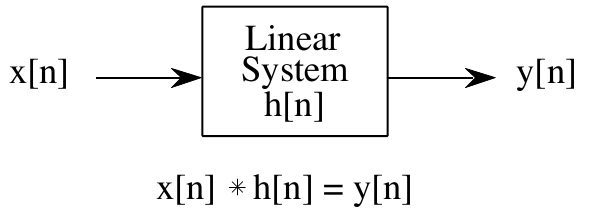
\includegraphics[width=0.492\linewidth,height=0.8\textheight,keepaspectratio]{assets/ch06/fig6-02.png}
\caption*{\textbf{图 6-2　DSP 中怎样使用卷积。}
线性系统的输出信号等于输入信号与系统冲激响应的卷积。写公式时，卷积用星号表示。}
\end{figure}

图 6-3
展示了用卷积做低通滤波和高通滤波。示例输入信号是两个分量之和：三个周期的正弦波（代表高频），加上一个缓慢上升的斜坡（由低频组成）。在
(a)
中，低通滤波器的冲激响应是一条平滑的拱形，结果只有缓慢变化的斜坡波形通过到输出。类似地，(b)
中的高通滤波器只让变化更快的正弦波通过。

\begin{figure}[htbp]
\centering
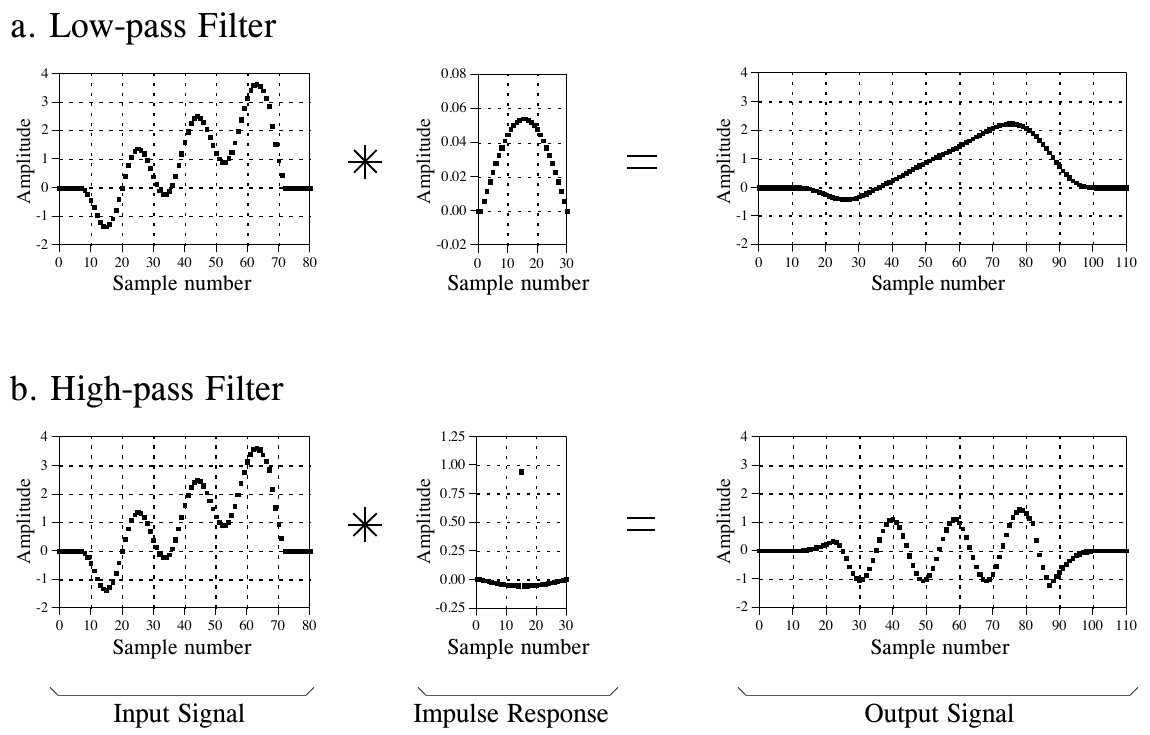
\includegraphics[width=0.958\linewidth,height=0.8\textheight,keepaspectratio]{assets/ch06/fig6-03.png}
\caption*{\textbf{图 6-3　用卷积做低通和高通滤波的例子。}
本例中，输入信号是几个周期的正弦波加上一个缓慢上升的斜坡。选取合适的冲激响应，就能把这两个分量分开。
（a. 低通滤波器(Low-pass Filter)；b. 高通滤波器(High-pass
Filter)。三栏依次为 Input Signal = 输入信号、Impulse Response =
冲激响应、Output Signal = 输出信号。Amplitude = 幅度，Sample number =
采样序号。）}
\end{figure}

图 6-4 给出了另外两个用卷积处理信号的例子。(a) 中的反相衰减器(inverting
attenuator)把信号上下翻转，并减小其幅度。(b) 中的离散导数(discrete
derivative，也叫一阶差分(first
difference))产生的输出信号与输入信号的斜率有关。

\begin{figure}[htbp]
\centering
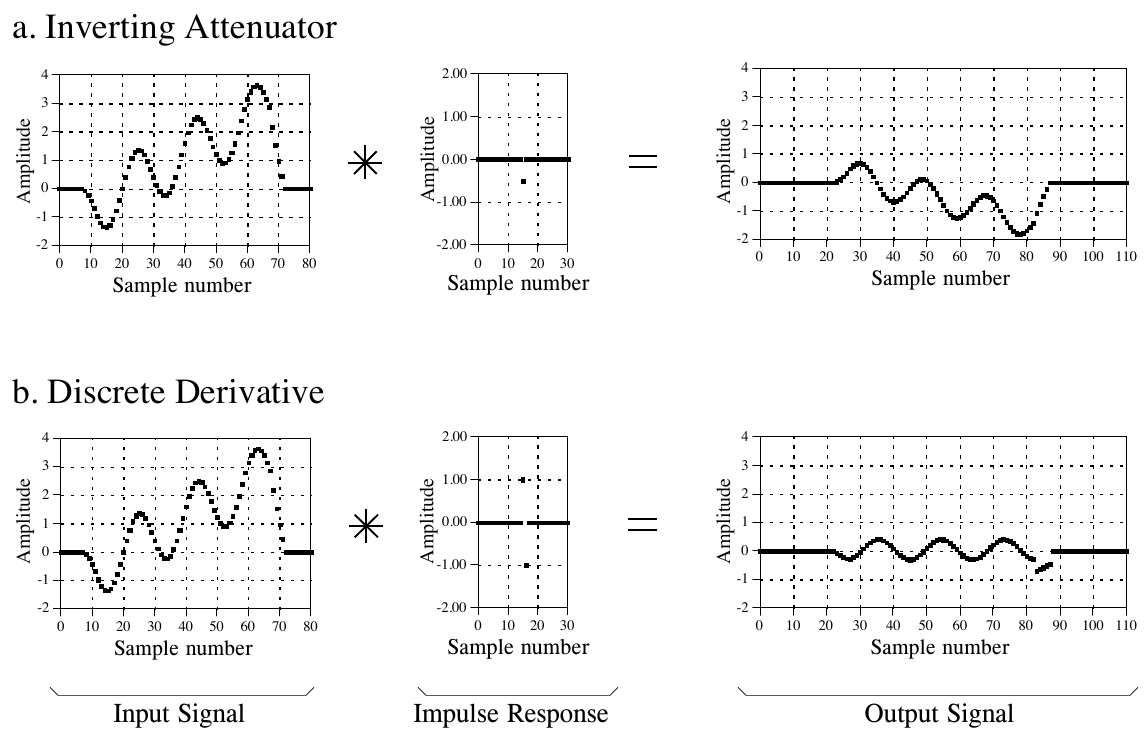
\includegraphics[width=0.954\linewidth,height=0.8\textheight,keepaspectratio]{assets/ch06/fig6-04.png}
\caption*{\textbf{图 6-4　用卷积处理信号的例子。}
许多信号处理任务用的冲激响应都非常简单。如这些例子所示，只用几个非零点就能产生显著的变化。
（a. 反相衰减器(Inverting Attenuator)；b. 离散导数(Discrete
Derivative)。三栏依次为输入信号、冲激响应、输出信号。）}
\end{figure}

注意图 6-3 和 6-4 中各信号的长度。输入信号长 81 个采样，每个冲激响应由
31 个采样组成。在大多数 DSP
应用中，输入信号长几百、几千甚至几百万个采样。冲激响应通常短得多，比如几个点到几百个点。卷积背后的数学并不限制这些信号有多长，但它确实规定了输出信号的长度：输出信号的长度等于输入信号的长度加上冲激响应的长度再减一。对于图
6-3 和 6-4 中的信号，每个输出信号长 81 + 31 − 1 = 111
个采样。输入信号从第 0 到第 80 个采样，冲激响应从第 0 到第 30
个采样，输出信号从第 0 到第 110 个采样。

现在来看卷积的详细数学。在数字信号处理中，卷积可以用两种不同的方式来理解。第一种从输入信号的角度看卷积：分析输入信号中的每个采样怎样影响输出信号中的许多点。第二种从输出信号的角度看卷积：考察输出信号中的每个采样怎样从输入信号的许多点接收信息。记住，这两个视角是对同一个数学运算的不同思考方式。第一个视角很重要，因为它提供了卷积与
DSP 有何关系的概念性理解。第二个视角描述了卷积的数学。这体现了你在 DSP
中会遇到的最难的任务之一：让你的概念性理解和用来交流这些想法的一堆数学对上号。

\section{输入端算法}

图 6-5 展示了一个简单的卷积问题：一个 9 点输入信号 x{[}n{]}
通过一个冲激响应为 4 点 h{[}n{]} 的系统，得到一个 9 + 4 − 1 = 12
点的输出信号 y{[}n{]}。用数学语言说，x{[}n{]} 与 h{[}n{]} 卷积得到
y{[}n{]}。卷积的第一个视角基于 DSP
的基本概念：分解输入，让各分量通过系统，再合成输出。在这个例子中，输入信号的九个采样中的每一个，都会给输出信号贡献一个经过缩放和平移的冲激响应。这九个信号如图
6-6 所示。把这九个信号相加，就得到输出信号 y{[}n{]}。

\begin{figure}[htbp]
\centering
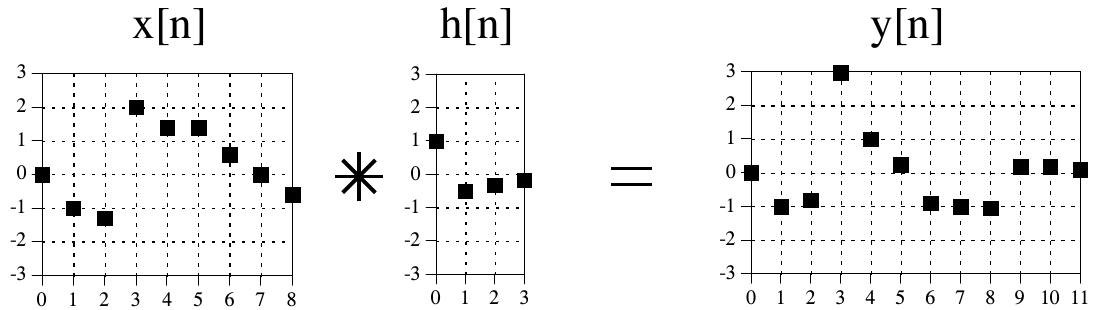
\includegraphics[width=0.912\linewidth,height=0.8\textheight,keepaspectratio]{assets/ch06/fig6-05.png}
\caption*{\textbf{图 6-5　卷积问题示例。}
一个九点的输入信号与一个四点的冲激响应卷积，得到一个十二点的输出信号。输入信号中的每个点都给输出信号贡献一个经过缩放和平移的冲激响应。这九个经过缩放和平移的冲激响应如图
6-6 所示。}
\end{figure}

我们详细看看这九个信号中的几个。先从输入信号的第 4 个采样，即 x{[}4{]}
开始。这个采样位于索引 4，值为 1.4。分解信号时，它变成一个冲激，表示为
\(1.4\,\delta[n-4]\)。通过系统后，得到的输出分量是
\(1.4\,h[n-4]\)。这个信号就是图 6-6
九个信号中正中间那个方框。注意，这是冲激响应 h{[}n{]} 乘以
1.4、再向右平移四个采样的结果。第 0～3 和第 8～11
个采样处补了零作为占位符。为了更清楚，图 6-6
用方块表示来自平移和缩放后冲激响应的数据点，用菱形表示补上的零。

现在看采样 x{[}8{]}，即输入信号的最后一个点。这个采样位于索引 8，值为
−0.5。如图 6-6 右下角的图所示，x{[}8{]} 产生一个向右平移八个点并乘以
−0.5 的冲激响应。第 0～7 点补了零作为占位符。最后，看看 x{[}0{]} 和
x{[}7{]}
这两个点的作用。这两个采样的值都为零，因此产生的输出分量全为零。

\begin{figure}[htbp]
\centering
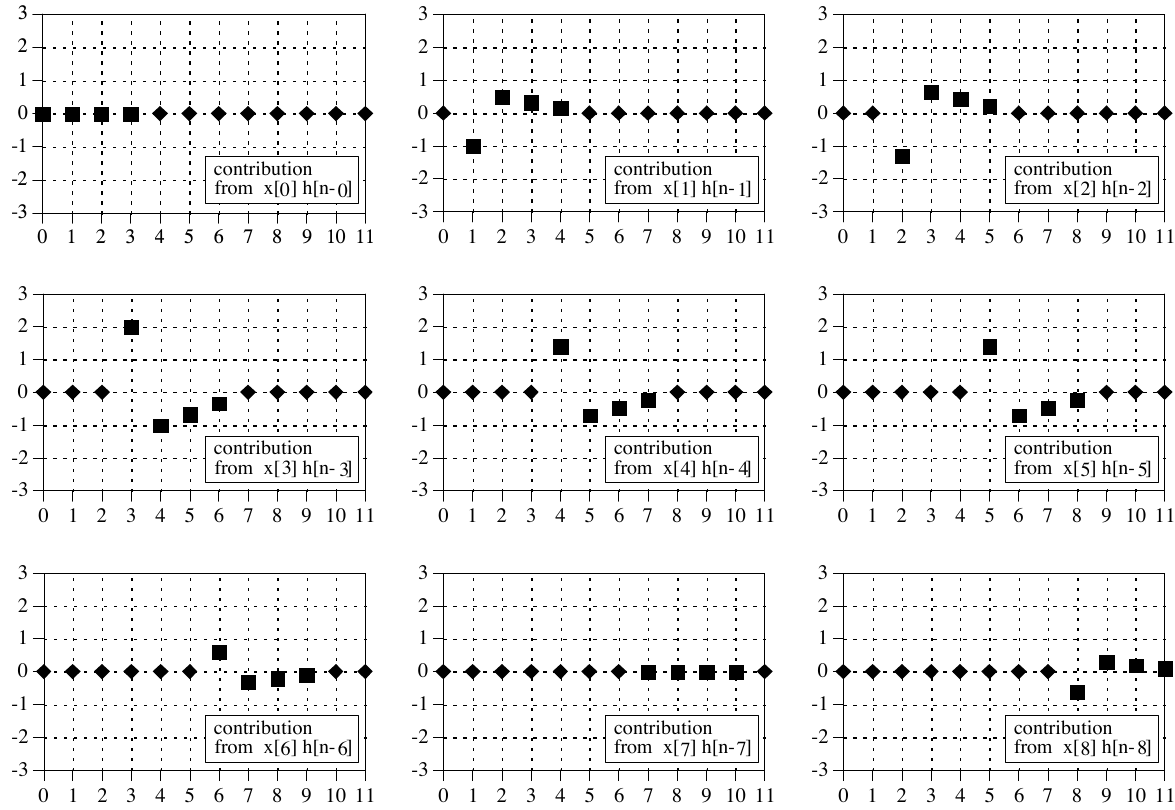
\includegraphics[width=0.979\linewidth,height=0.8\textheight,keepaspectratio]{assets/ch06/fig6-06.png}
\caption*{\textbf{图 6-6　图 6-5 卷积的输出信号分量。}
在这些信号中，来自缩放和平移后冲激响应的点用方块标记表示。其余的数据点用菱形表示，是作为占位符补上的零。
（contribution from x{[}k{]} h{[}n−k{]} = 由 x{[}k{]} 贡献的
h{[}n−k{]}，k = 0～8。）}
\end{figure}

在这个例子中，x{[}n{]} 是九点信号，h{[}n{]} 是四点信号。在下一个例子（图
6-7）中，我们把情况反过来：让 x{[}n{]} 是四点信号，h{[}n{]}
是九点信号。用的还是这两个波形，只是交换了一下。从输出信号分量可以看出，x{[}n{]}
的四个采样产生了九点冲激响应的四个经过平移和缩放的版本。和前面一样，前后补零作为占位符。

等一下！图 6-7 的输出信号和图 6-5
的输出信号完全相同。这不是错误，而是一个重要的性质：卷积满足交换律(commutative)，\(a[n] * b[n] = b[n] * a[n]\)。数学并不在乎哪个是输入信号、哪个是冲激响应，只在乎两个信号相互卷积。数学虽然允许这样做，但在系统理论中交换这两个信号没有物理意义。输入信号和冲激响应是完全不同的两样东西，交换它们说不通。交换律提供的是一个数学工具，用来变换公式以得到各种结果。

\begin{figure}[htbp]
\centering
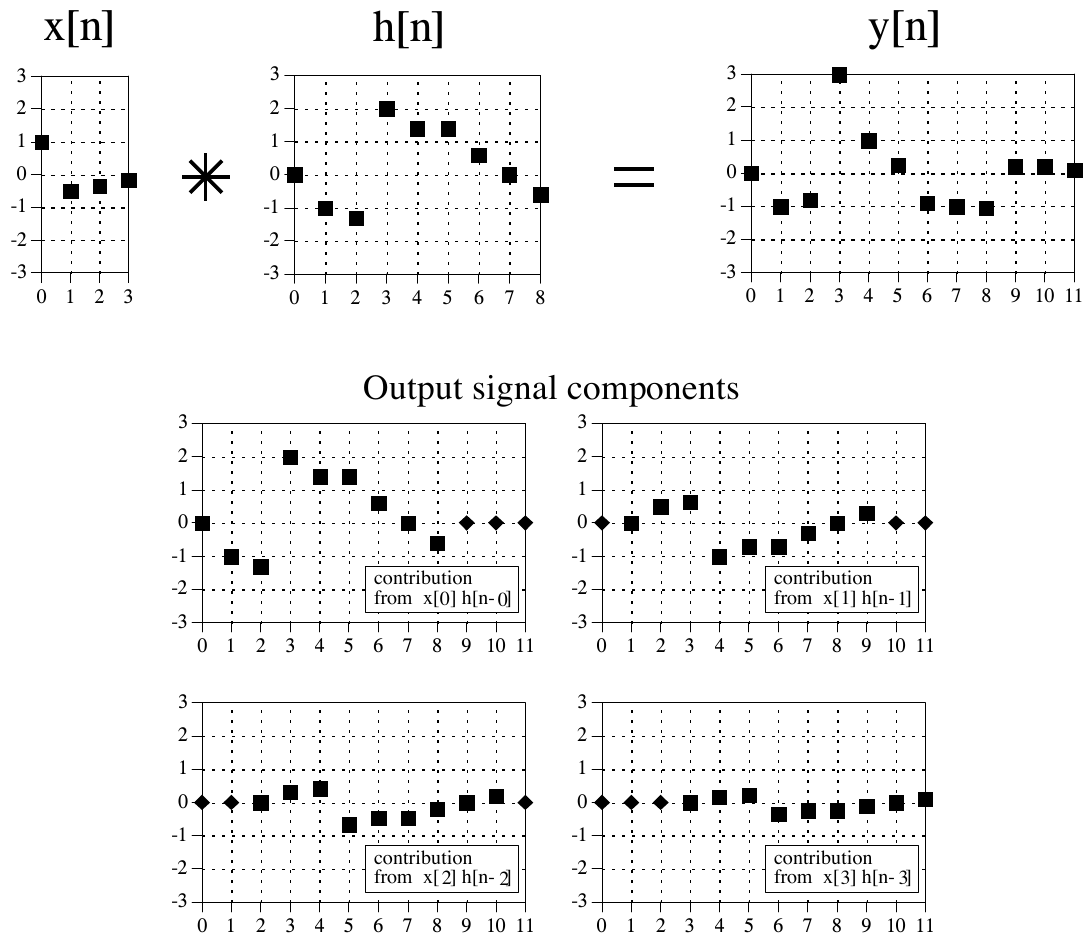
\includegraphics[width=0.908\linewidth,height=0.8\textheight,keepaspectratio]{assets/ch06/fig6-07.png}
\caption*{\textbf{图 6-7　卷积的第二个例子。} 输入信号和冲激响应的波形与图 6-5
的例子互换了。由于卷积满足交换律，两个例子的输出信号完全相同。 （Output
signal components = 输出信号分量。）}
\end{figure}

表 6-1
是一个用输入端算法计算卷积的程序。记住，本书的程序旨在以最简单的形式传达算法，哪怕牺牲良好的编程风格。例如，所有输入和输出都在虚构的子程序（第
160 和 280
行）中处理，也就是说，我们并不定义这些操作具体怎样进行。不要跳过这些程序，它们是内容的关键部分，你需要详细理解。

这个程序把存放在数组 X{[} {]} 中的 81 点输入信号，与存放在数组 H{[} {]}
中的 31 点冲激响应卷积，得到存放在数组 Y{[} {]} 中的 111
点输出信号。这和图 6-3、6-4
中的长度相同。注意这些数组名用的是大写字母。这违反了前面讲的命名约定，因为大写字母是留给频域信号的。可惜本书用的简单
BASIC 不允许小写变量名。还要注意，第 240
行用星号表示乘法。记住，程序里的星号表示乘法，公式里的星号表示卷积。文字（比如文档或程序注释）中的星号两者都可能。

第 160 行的虚构子程序把输入信号放进 X{[} {]}，把冲激响应放进 H{[}
{]}。第 180～200 行把 Y{[} {]} 的所有值设为零。这是必要的，因为 Y{[} {]}
被用作累加器，在计算输出分量的过程中把它们加起来。第 220～260
行是程序的核心。第 220 行的 FOR 语句控制一个循环，逐个遍历输入信号 X{[}
{]} 中的每个点。对输入信号中的每个采样，内层循环（第 230～250
行）计算冲激响应的一个经过缩放和平移的版本，并把它加到累积输出信号的数组
Y{[} {]}
中。这种嵌套循环结构（一个循环套在另一个循环里）是卷积程序的一个关键特征，要熟悉它。

\textbf{表 6-1}（注释已译成中文）

\begin{Shaded}
\begin{Highlighting}[]
\NormalTok{100 \textquotesingle{}CONVOLUTION USING THE INPUT SIDE ALGORITHM}
\NormalTok{110 \textquotesingle{}}
\NormalTok{120 DIM X[80]                   \textquotesingle{}输入信号，81 点}
\NormalTok{130 DIM H[30]                   \textquotesingle{}冲激响应，31 点}
\NormalTok{140 DIM Y[110]                  \textquotesingle{}输出信号，111 点}
\NormalTok{150 \textquotesingle{}}
\NormalTok{160 GOSUB XXXX                  \textquotesingle{}虚构的子程序，载入 X[ ] 和 H[ ]}
\NormalTok{170 \textquotesingle{}}
\NormalTok{180 FOR I\% = 0 TO 110           \textquotesingle{}把输出数组清零}
\NormalTok{190   Y(I\%) = 0}
\NormalTok{200 NEXT I\%}
\NormalTok{210 \textquotesingle{}}
\NormalTok{220 FOR I\% = 0 TO 80            \textquotesingle{}遍历 X[ ] 中的每个点}
\NormalTok{230   FOR J\% = 0 TO 30          \textquotesingle{}遍历 H[ ] 中的每个点}
\NormalTok{240     Y[I\%+J\%] = Y[I\%+J\%] + X[I\%]*H[J\%]}
\NormalTok{250   NEXT J\%}
\NormalTok{260 NEXT I\%                     \textquotesingle{}（记住，程序里的 * 是乘法！）}
\NormalTok{270 \textquotesingle{}}
\NormalTok{280 GOSUB XXXX                  \textquotesingle{}虚构的子程序，保存 Y[ ]}
\NormalTok{290 \textquotesingle{}}
\NormalTok{300 END}
\end{Highlighting}
\end{Shaded}

\textbf{C 实现}（完整可编译版本见
\texttt{c/table6-1\_convolve\_input\_side.c}，其中用图 6-3a
的设定生成了输入信号和低通冲激响应）：

\begin{Shaded}
\begin{Highlighting}[]
\PreprocessorTok{\#define NX }\DecValTok{81}\PreprocessorTok{                   }\CommentTok{/* 120 DIM X[80]：输入信号 81 点 */}
\PreprocessorTok{\#define NH }\DecValTok{31}\PreprocessorTok{                   }\CommentTok{/* 130 DIM H[30]：冲激响应 31 点 */}
\PreprocessorTok{\#define NY }\OperatorTok{(}\PreprocessorTok{NX }\OperatorTok{+}\PreprocessorTok{ NH }\OperatorTok{{-}}\PreprocessorTok{ }\DecValTok{1}\OperatorTok{)}\PreprocessorTok{        }\CommentTok{/* 140 DIM Y[110]：输出信号 111 点 */}

\CommentTok{/* 输入端算法：输入的每个点，都往输出里加一份缩放、平移后的冲激响应 */}
\DataTypeTok{static} \DataTypeTok{void}\NormalTok{ convolve\_input\_side}\OperatorTok{(}\DataTypeTok{const} \DataTypeTok{double} \OperatorTok{*}\NormalTok{x}\OperatorTok{,} \DataTypeTok{const} \DataTypeTok{double} \OperatorTok{*}\NormalTok{h}\OperatorTok{,} \DataTypeTok{double} \OperatorTok{*}\NormalTok{y}\OperatorTok{)}
\OperatorTok{\{}
    \ControlFlowTok{for} \OperatorTok{(}\DataTypeTok{int}\NormalTok{ i }\OperatorTok{=} \DecValTok{0}\OperatorTok{;}\NormalTok{ i }\OperatorTok{\textless{}}\NormalTok{ NY}\OperatorTok{;}\NormalTok{ i}\OperatorTok{++)}        \CommentTok{/* 180～200：输出数组清零，后面当累加器用 */}
\NormalTok{        y}\OperatorTok{[}\NormalTok{i}\OperatorTok{]} \OperatorTok{=} \FloatTok{0.0}\OperatorTok{;}

    \ControlFlowTok{for} \OperatorTok{(}\DataTypeTok{int}\NormalTok{ i }\OperatorTok{=} \DecValTok{0}\OperatorTok{;}\NormalTok{ i }\OperatorTok{\textless{}}\NormalTok{ NX}\OperatorTok{;}\NormalTok{ i}\OperatorTok{++)}        \CommentTok{/* 220：遍历输入的每个点 */}
        \ControlFlowTok{for} \OperatorTok{(}\DataTypeTok{int}\NormalTok{ j }\OperatorTok{=} \DecValTok{0}\OperatorTok{;}\NormalTok{ j }\OperatorTok{\textless{}}\NormalTok{ NH}\OperatorTok{;}\NormalTok{ j}\OperatorTok{++)}    \CommentTok{/* 230：遍历冲激响应的每个点 */}
\NormalTok{            y}\OperatorTok{[}\NormalTok{i }\OperatorTok{+}\NormalTok{ j}\OperatorTok{]} \OperatorTok{+=}\NormalTok{ x}\OperatorTok{[}\NormalTok{i}\OperatorTok{]} \OperatorTok{*}\NormalTok{ h}\OperatorTok{[}\NormalTok{j}\OperatorTok{];}    \CommentTok{/* 240：缩放（乘 x[i]）、平移（下标 +i）、累加 */}
\OperatorTok{\}}
\end{Highlighting}
\end{Shaded}

第 240 行的下标很容易把人绕晕！假设程序执行到一半，刚开始处理采样
X{[}40{]}，即 I\% =
40。内层循环遍历冲激响应的每个点，做三件事。第一，把冲激响应乘以这个输入采样的值来缩放。如果内层循环只做这一件事，第
240 行可以写成
\texttt{Y{[}J\%{]}\ =\ X{[}40{]}*H{[}J\%{]}}。第二，给输出信号所用的下标加上
40，把缩放后的冲激响应向右平移 40 个采样。这第二个动作会把第 240 行变成
\texttt{Y{[}40+J\%{]}\ =\ X{[}40{]}*H{[}J\%{]}}。第三，Y{[} {]}
必须累加（合成）输入信号中每个采样产生的所有信号。因此，新信息必须加到数组中已有的信息上。于是得到最终的命令：\texttt{Y{[}40+J\%{]}\ =\ Y{[}40+J\%{]}\ +\ X{[}40{]}*H{[}J\%{]}}。仔细研究一下，它非常绕，但非常重要。

\section{输出端算法}

卷积的第一个视角分析的是输入信号中的每个采样怎样影响输出信号中的许多采样。在第二个视角中，我们反过来：看输出信号中的单个采样，找出输入中对它有贡献的点。无论从数学还是实用的角度看，这都很重要。假设给定某个输入信号和冲激响应，要求两者的卷积。最直接的方法是写一个程序遍历输出信号，每次循环算出一个采样。同样，公式也写成这样的形式：y{[}n{]}
= 其他变量的某种组合。也就是说，输出信号的第 n
个采样等于输入信号和冲激响应中许多值的某种组合。这要求我们知道输出信号中的每个采样怎样独立于输出信号中所有其他采样计算出来。输出端算法提供的正是这个信息。

我们来看一个例子，看输出信号中的单个点怎样受输入中几个点的影响。我们用图
6-5 中的 y{[}6{]} 作例子。这个点等于图 6-6 中九个输出分量的第 6
个点之和。现在仔细看这九个输出分量，找出哪些能影响
y{[}6{]}，即这九个信号中哪些在第 6
个位置上有非零采样。有五个输出分量在第 6
个采样处只有补上的零（菱形标记），因此可以忽略。只有四个输出分量可能在第
6 个位置上有非零值。它们是由输入采样 x{[}3{]}、x{[}4{]}、x{[}5{]} 和
x{[}6{]} 产生的输出分量。把这些输出分量的第 6 个采样加起来，就确定了
y{[}6{]}：\(y[6] = x[3]h[3] + x[4]h[2] + x[5]h[1] + x[6]h[0]\)。也就是说，输入信号的四个采样与冲激响应的四个采样相乘，再把乘积相加。

图 6-8 把输出端算法画成了一台卷积机(convolution
machine)，即卷积怎样发生的流程图。把输入信号 x{[}n{]} 和输出信号
y{[}n{]}
想象成固定在纸面上。卷积机，即虚线框内的一切，可以根据需要左右自由移动。卷积机的位置让它的输出对准正在计算的那个输出采样。输入信号的四个采样落进卷积机的输入端，这些值乘以冲激响应中标出的采样，再把乘积相加。这就得到输出信号的值，它落到正确的位置上。例如，图中正在用四个输入采样
x{[}3{]}、x{[}4{]}、x{[}5{]} 和 x{[}6{]} 计算 y{[}6{]}。

要计算 y{[}7{]}，卷积机向右移动一个采样。这样另外四个采样 x{[}4{]} 到
x{[}7{]} 进入机器，y{[}7{]}
的值落到正确的位置上。对输出信号中所有需要计算的点重复这个过程。

\begin{figure}[htbp]
\centering
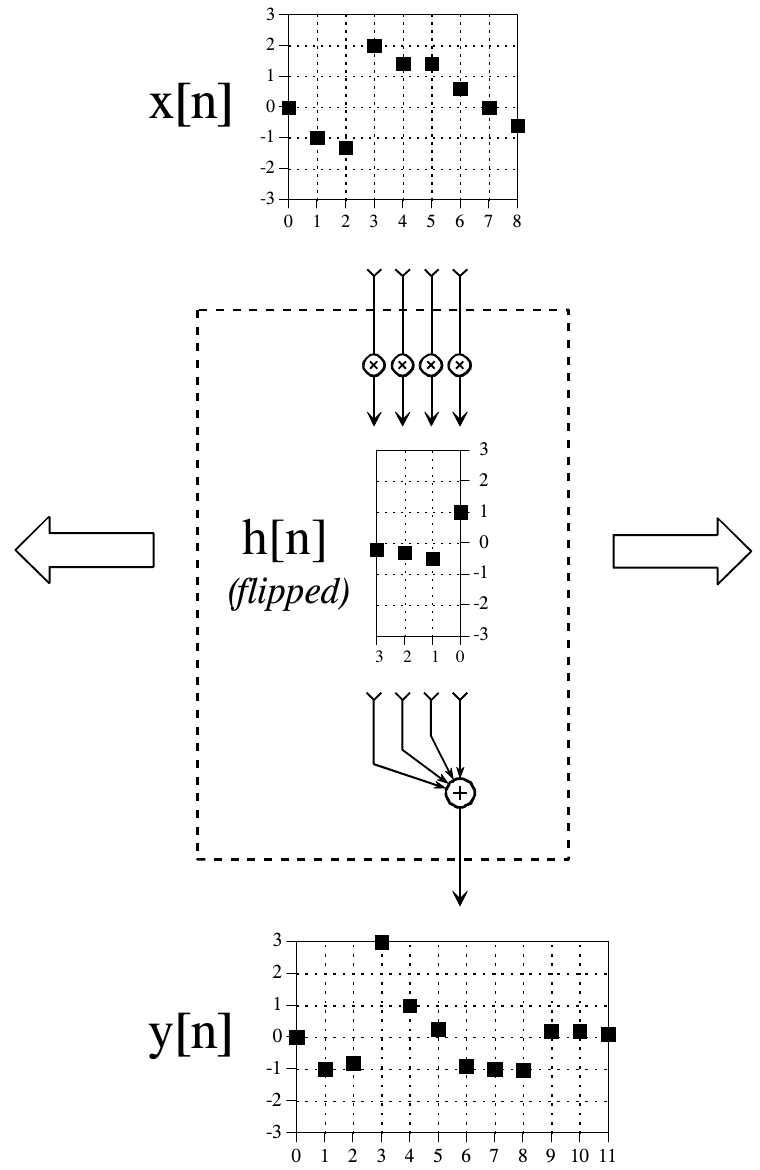
\includegraphics[width=0.633\linewidth,height=0.8\textheight,keepaspectratio]{assets/ch06/fig6-08.png}
\caption*{\textbf{图 6-8　卷积机。}
这是一张流程图，显示输出信号中的每个采样怎样受输入信号和冲激响应的影响。详见正文。
（h{[}n{]} (flipped) = 翻转后的 h{[}n{]}。）}
\end{figure}

冲激响应在卷积机中的排列非常重要：冲激响应是左右翻转的。这样第 0
个采样在最右边，采样序号越大越往左。把它和图 6-5
中正常的冲激响应比较一下，就能理解这种翻转的几何关系。为什么需要翻转？它只是从数学中自然推出来的。冲激响应描述的是输入信号中的每个点怎样影响输出信号。这导致输出信号中的每个点，受到的是输入信号中的点按翻转后的冲激响应加权的影响。

图 6-9
展示了用卷积机计算输出信号中的几个采样。这张图也说明了卷积中一个真正的麻烦。在
(a) 中，卷积机位于最左边，输出对准 y{[}0{]}。在这个位置，它试图从采样
x{[}−3{]}、x{[}−2{]}、x{[}−1{]} 和 x{[}0{]}
接收输入。问题是，其中三个采样 x{[}−3{]}、x{[}−2{]} 和 x{[}−1{]}
并不存在！同样的困境也出现在 (d)
中，卷积机试图接收已定义输入信号右边的采样，即 x{[}9{]}、x{[}10{]} 和
x{[}11{]}。

\begin{figure}[htbp]
\centering
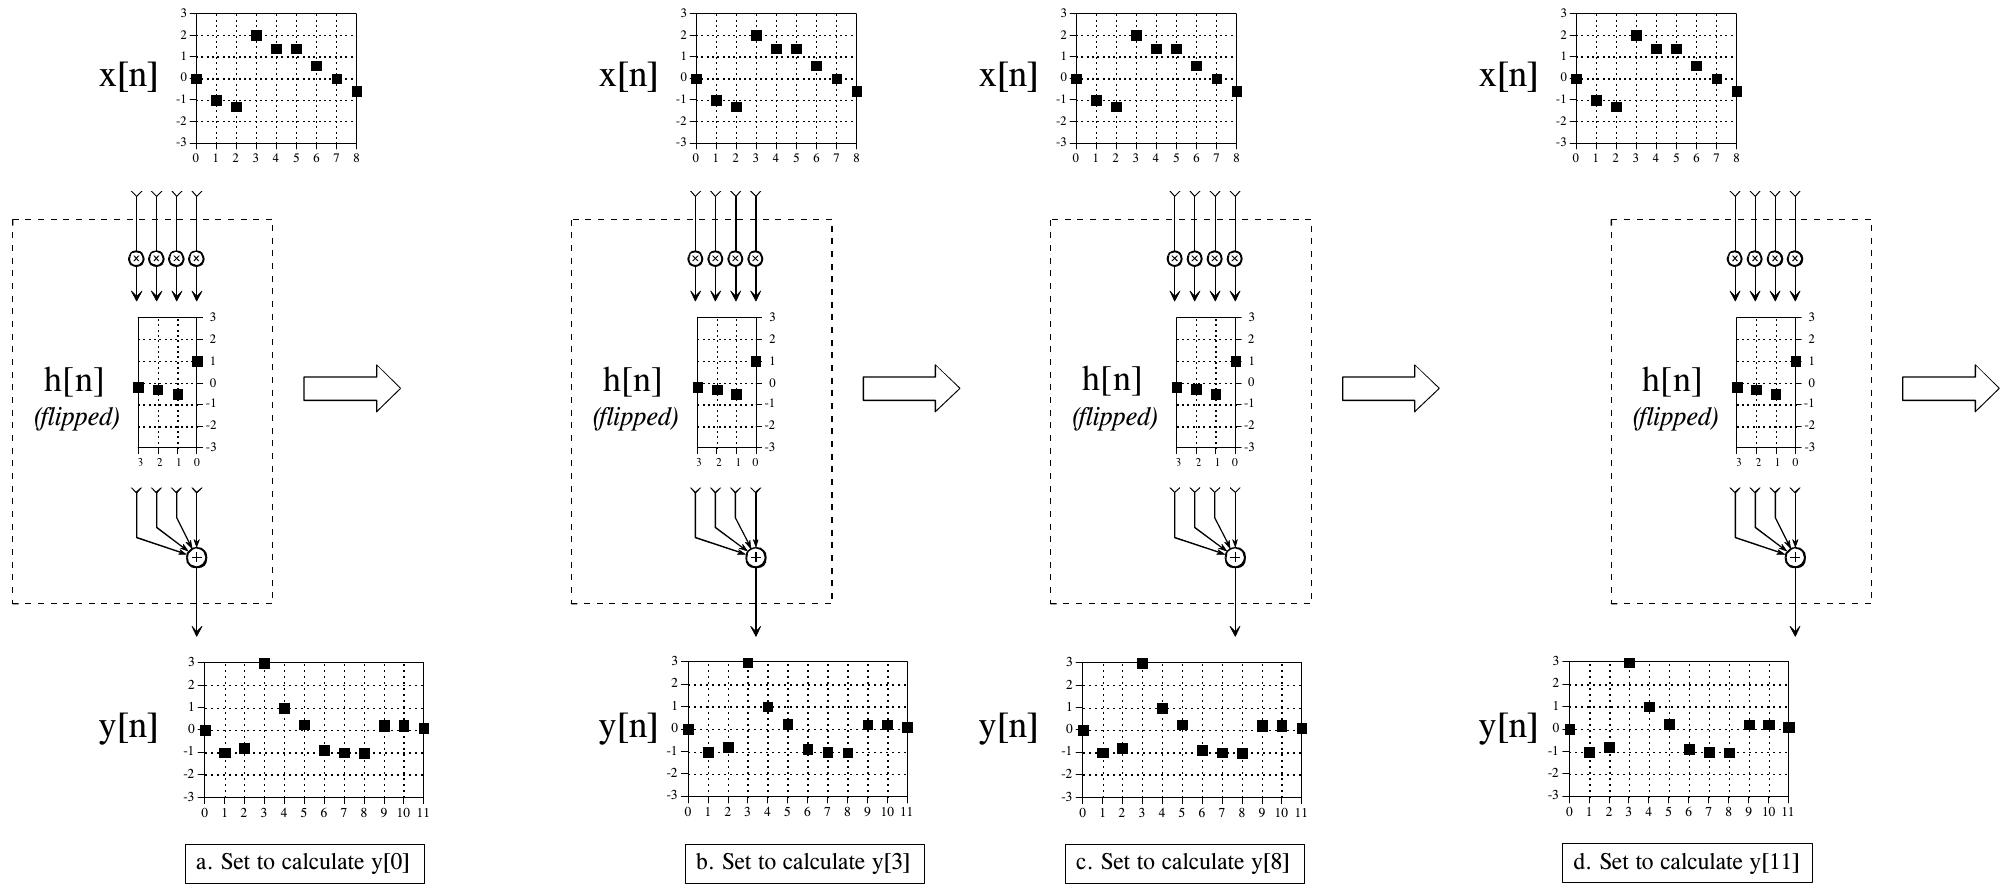
\includegraphics[width=1.000\linewidth,height=0.8\textheight,keepaspectratio]{assets/ch06/fig6-09.png}
\caption*{\textbf{图 6-9　卷积机在工作。} 图 (a)～(d)
显示卷积机分别设置为计算四个不同的输出采样：y{[}0{]}、y{[}3{]}、y{[}8{]}
和 y{[}11{]}。 （a. 设置为计算 y{[}0{]}；b. 设置为计算
y{[}3{]}；c.~设置为计算 y{[}8{]}；d.~设置为计算 y{[}11{]}。原书 (c)(d)
在下一页，这里拼成一张。）}
\end{figure}

处理这个问题的一种办法是把不存在的采样「造」出来。做法是在输入信号的两端添加采样，每个添加的采样值都为零。这叫给信号补零(padding
the signal with
zeros)。卷积机不再试图访问不存在的值，而是收到一个值为零的采样。由于这个零在乘法中被消掉了，结果在数学上和忽略不存在的输入是一样的。

重要的是，输出信号最左边和最右边的采样是基于不完整的信息算出来的。用 DSP
的行话说，冲激响应没有完全浸没(fully
immersed)在输入信号中。如果冲激响应长 M 点，输出信号的前 M−1 个和后 M−1
个采样所依据的信息比中间的采样少。这就像电子电路通电后需要一段时间才能稳定下来。区别在于，这种瞬态(transient)在电子学中很容易忽略，在
DSP 中却非常突出。

图 6-10 展示了这些端点效应(end
effects)可能造成的麻烦。输入信号是一个正弦波加上一个直流分量。目的是去掉信号的直流部分，同时保留正弦波。这需要一个高通滤波器，比如图中所示的冲激响应。问题是，前
30 个和后 30 个点一团糟！要理解这些端区的形状，可以想象输入信号左边补了
30 个零（采样 x{[}−1{]} 到 x{[}−30{]}），右边补了 30 个零（采样
x{[}81{]} 到
x{[}110{]}）。这样输出信号就可以看作对这个更长波形的滤波结果。这种「端点效应」问题在
DSP 中很普遍。一般来说，预计处理后信号开头和结尾的采样会相当没用。

\begin{figure}[htbp]
\centering
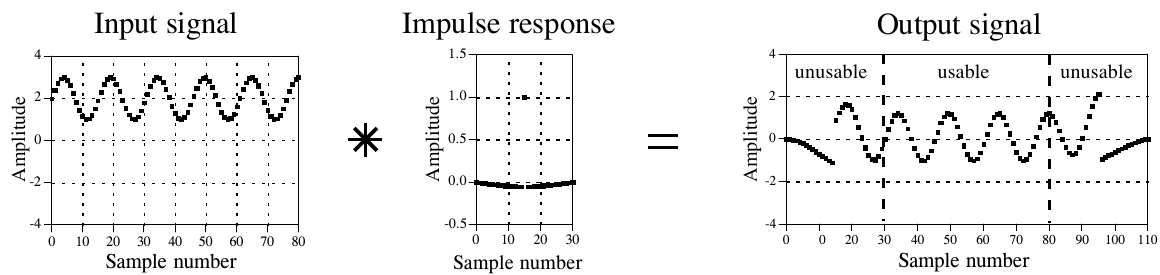
\includegraphics[width=0.967\linewidth,height=0.8\textheight,keepaspectratio]{assets/ch06/fig6-10.png}
\caption*{\textbf{图 6-10　卷积中的端点效应。} 输入信号与 M
点冲激响应卷积时，输出信号的前 M−1 个和后 M−1
个点可能无法使用。本例中，冲激响应是一个高通滤波器，用来去掉输入信号中的直流分量。
（Input signal = 输入信号，Impulse response = 冲激响应，Output signal =
输出信号，usable = 可用，unusable = 不可用。）}
\end{figure}

现在讲数学。以卷积机为指导，我们可以写出卷积的标准公式。如果 x{[}n{]}
是从 0 到 N−1 的 N 点信号，h{[}n{]} 是从 0 到 M−1 的 M
点信号，两者的卷积 \(y[n] = x[n] * h[n]\) 是一个从 0 到 N+M−2 的 N+M−1
点信号，由下式给出：

\textbf{公式 6-1　卷积和。} 这是卷积的正式定义，简写为
\(y[n] = x[n] * h[n]\)。式中 h{[}n{]} 是一个 M 点信号，索引从 0 到 M−1。

\[
y[i] = \sum_{j=0}^{M-1} h[j]\, x[i-j]
\]

这个公式叫卷积和(convolution
sum)。它让输出信号中的每个点都能独立于输出信号中的所有其他点计算出来。索引
i
决定正在计算输出信号的哪个采样，因此对应卷积机的左右位置。在执行卷积的计算机程序中，用一个循环让这个索引遍历输出信号的每个采样。计算其中一个输出采样时，在卷积机内部使用索引
j。当 j 从 0 走到 M−1 时，冲激响应中的每个采样 h{[}j{]}
都乘以输入信号中相应的采样
x{[}i−j{]}。把所有这些乘积相加，就得到正在计算的那个输出采样。仔细研究公式
6-1，直到你完全理解卷积机是怎样实现它的。DSP
的很多内容都基于这个公式。（不要被 \(y[n] = x[n] * h[n]\) 中的 n
搞糊涂。它只是一个占位符，表示某个变量是数组的索引。有时公式写成
\(y[\,] = x[\,] * h[\,]\)，就是为了避免引入一个没有意义的符号。）

表 6-2 是用输出端算法做卷积的程序，直接实现了公式
6-1。这个程序产生的输出信号和前面表 6-1
的输入端算法程序相同。注意这两个程序的主要区别：输入端算法遍历输入信号的每个采样（表
6-1 第 220 行），而输出端算法遍历输出信号的每个采样（表 6-2 第 180
行）。

下面详细说明这个程序的运作。第 180～250 行的 FOR-NEXT 循环用 I\%
作索引，遍历输出信号的每个采样。对其中每个值，由第 200～230
行组成的内层循环计算输出采样 Y{[}I\%{]} 的值。第 190 行把 Y{[}I\%{]}
设为零，让它累加卷积机内部的乘积。第 200～240 行的 FOR-NEXT
循环直接实现了公式 6-1。索引 J\% 遍历冲激响应的每个采样。第 230
行把冲激响应的每个采样 H{[}J\%{]} 与输入信号中相应的采样 X{[}I\%-J\%{]}
相乘，并把结果加到累加器上。

第 230 行从输入信号中取的采样是 X{[}I\%-J\%{]}。第 210 和 220
行防止它超出已定义的数组 X{[}0{]} 到
X{[}80{]}。换句话说，这个程序对输入信号中未定义的采样的处理方式是忽略它们。另一种办法是把输入信号的数组定义为
X{[}-30{]} 到 X{[}110{]}，在真实数据两侧各补 30 个零。第三种办法是把第
180 行的 FOR-NEXT 循环改成从 30 到 80，而不是从 0 到
110。也就是说，程序只计算输出信号中冲激响应完全浸没在输入信号中的那些采样。重要的是，你必须使用这三种技术之一。否则，程序试图读取越界数据时就会崩溃。

\textbf{表 6-2}（注释已译成中文）

\begin{Shaded}
\begin{Highlighting}[]
\NormalTok{100 \textquotesingle{}CONVOLUTION USING THE OUTPUT SIDE ALGORITHM}
\NormalTok{110 \textquotesingle{}}
\NormalTok{120 DIM X[80]                   \textquotesingle{}输入信号，81 点}
\NormalTok{130 DIM H[30]                   \textquotesingle{}冲激响应，31 点}
\NormalTok{140 DIM Y[110]                  \textquotesingle{}输出信号，111 点}
\NormalTok{150 \textquotesingle{}}
\NormalTok{160 GOSUB XXXX                  \textquotesingle{}虚构的子程序，载入 X[ ] 和 H[ ]}
\NormalTok{170 \textquotesingle{}}
\NormalTok{180 FOR I\% = 0 TO 110           \textquotesingle{}遍历 Y[ ] 中的每个点}
\NormalTok{190   Y[I\%] = 0                 \textquotesingle{}把输出数组中的这个采样清零}
\NormalTok{200   FOR J\% = 0 TO 30          \textquotesingle{}遍历 H[ ] 中的每个点}
\NormalTok{210     IF (I\%{-}J\% \textless{} 0)  THEN GOTO 240}
\NormalTok{220     IF (I\%{-}J\% \textgreater{} 80) THEN GOTO 240}
\NormalTok{230     Y(I\%) = Y(I\%) + H(J\%)*X(I\%{-}J\%)}
\NormalTok{240   NEXT J\%}
\NormalTok{250 NEXT I\%}
\NormalTok{260 \textquotesingle{}}
\NormalTok{270 GOSUB XXXX                  \textquotesingle{}虚构的子程序，保存 Y[ ]}
\NormalTok{280 \textquotesingle{}}
\NormalTok{290 END}
\end{Highlighting}
\end{Shaded}

\textbf{C 实现}（完整可编译版本见
\texttt{c/table6-2\_convolve\_output\_side.c}，信号与表 6-1 的 C
版本相同，两者输出逐点一致）：

\begin{Shaded}
\begin{Highlighting}[]
\PreprocessorTok{\#define NX }\DecValTok{81}\PreprocessorTok{                   }\CommentTok{/* 120 DIM X[80]：输入信号 81 点 */}
\PreprocessorTok{\#define NH }\DecValTok{31}\PreprocessorTok{                   }\CommentTok{/* 130 DIM H[30]：冲激响应 31 点 */}
\PreprocessorTok{\#define NY }\OperatorTok{(}\PreprocessorTok{NX }\OperatorTok{+}\PreprocessorTok{ NH }\OperatorTok{{-}}\PreprocessorTok{ }\DecValTok{1}\OperatorTok{)}\PreprocessorTok{        }\CommentTok{/* 140 DIM Y[110]：输出信号 111 点 */}

\CommentTok{/* 输出端算法：公式 6{-}1 的直接实现，每个输出点独立算出 */}
\DataTypeTok{static} \DataTypeTok{void}\NormalTok{ convolve\_output\_side}\OperatorTok{(}\DataTypeTok{const} \DataTypeTok{double} \OperatorTok{*}\NormalTok{x}\OperatorTok{,} \DataTypeTok{const} \DataTypeTok{double} \OperatorTok{*}\NormalTok{h}\OperatorTok{,} \DataTypeTok{double} \OperatorTok{*}\NormalTok{y}\OperatorTok{)}
\OperatorTok{\{}
    \ControlFlowTok{for} \OperatorTok{(}\DataTypeTok{int}\NormalTok{ i }\OperatorTok{=} \DecValTok{0}\OperatorTok{;}\NormalTok{ i }\OperatorTok{\textless{}}\NormalTok{ NY}\OperatorTok{;}\NormalTok{ i}\OperatorTok{++)} \OperatorTok{\{}          \CommentTok{/* 180：遍历输出的每个点 */}
\NormalTok{        y}\OperatorTok{[}\NormalTok{i}\OperatorTok{]} \OperatorTok{=} \FloatTok{0.0}\OperatorTok{;}                         \CommentTok{/* 190：这个输出点的累加器清零 */}
        \ControlFlowTok{for} \OperatorTok{(}\DataTypeTok{int}\NormalTok{ j }\OperatorTok{=} \DecValTok{0}\OperatorTok{;}\NormalTok{ j }\OperatorTok{\textless{}}\NormalTok{ NH}\OperatorTok{;}\NormalTok{ j}\OperatorTok{++)} \OperatorTok{\{}      \CommentTok{/* 200：遍历冲激响应的每个点 */}
            \ControlFlowTok{if} \OperatorTok{(}\NormalTok{i }\OperatorTok{{-}}\NormalTok{ j }\OperatorTok{\textless{}} \DecValTok{0}\OperatorTok{)} \ControlFlowTok{continue}\OperatorTok{;}        \CommentTok{/* 210～220：x[i{-}j] 越界的项不存在，跳过 */}
            \ControlFlowTok{if} \OperatorTok{(}\NormalTok{i }\OperatorTok{{-}}\NormalTok{ j }\OperatorTok{\textgreater{}}\NormalTok{ NX }\OperatorTok{{-}} \DecValTok{1}\OperatorTok{)} \ControlFlowTok{continue}\OperatorTok{;}
\NormalTok{            y}\OperatorTok{[}\NormalTok{i}\OperatorTok{]} \OperatorTok{+=}\NormalTok{ h}\OperatorTok{[}\NormalTok{j}\OperatorTok{]} \OperatorTok{*}\NormalTok{ x}\OperatorTok{[}\NormalTok{i }\OperatorTok{{-}}\NormalTok{ j}\OperatorTok{];}        \CommentTok{/* 230：h[j]·x[i{-}j]，即卷积机里的一次乘加 */}
        \OperatorTok{\}}
    \OperatorTok{\}}
\OperatorTok{\}}
\end{Highlighting}
\end{Shaded}

\section{输入的加权求和}

线性系统的特性完全由它的冲激响应描述。这是输入端算法的基础：输入信号中的每个点都给输出信号贡献一个经过缩放和平移的冲激响应。由此推出的数学结果就是输出端算法：输出信号中的每个点都从输入信号的许多点接收贡献，这些点乘以翻转后的冲激响应。这些虽然都对，但并没有完整说明卷积为什么在信号处理中这么重要。

回头看图 6-8
中的卷积机，先别管虚线框里的信号是冲激响应。把它看作一组碰巧嵌在流程图里的加权系数(weighing
coefficients)。从这个角度看，输出信号中的每个采样都等于输入的加权和(sum
of weighted
inputs)。输出中的每个采样受输入信号中一片区域的采样影响，这片区域由选定的加权系数决定。例如，设想有十个加权系数，每个都是十分之一。这样输出信号中的每个采样就是输入中十个采样的平均值。

更进一步，加权系数并不一定只能在正在计算的输出采样的左边。例如，图 6-8
显示 y{[}6{]} 是由 x{[}3{]}、x{[}4{]}、x{[}5{]} 和 x{[}6{]}
算出来的。把卷积机看作输入的加权和时，加权系数可以选得围绕输出采样对称。例如，y{[}6{]}
可以从 x{[}4{]}、x{[}5{]}、x{[}6{]}、x{[}7{]} 和 x{[}8{]}
接收贡献。按照图 6-8 中同样的索引记法，这五个输入的加权系数存放在
h{[}2{]}、h{[}1{]}、h{[}0{]}、h{[}−1{]} 和 h{[}−2{]}
中。换句话说，对应我们所选的对称加权系数的冲激响应，需要使用负索引。下一章我们会回到这个问题。

从数学上说，这里只有一个概念：公式 6-1
定义的卷积。然而，科学和工程问题从两个截然不同的方向接近这同一个概念。有时你会想从系统的冲激响应长什么样来思考系统；另一些时候，你会把系统理解为一组加权系数。你需要熟悉这两种视角，以及怎样在它们之间切换。
